\documentclass[tikz]{standalone}
\usetikzlibrary{positioning,automata}

\begin{document}
    \centering
    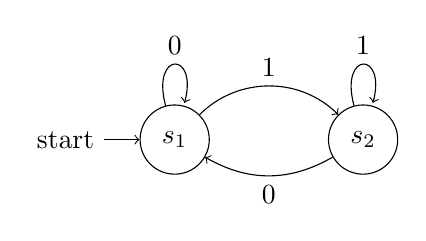
\begin{tikzpicture}[node distance = 1.5cm, auto]
        % Place nodes
        \node[state,initial]   (s_1)                {$s_1$};
        \node[state]           (s_2) [right=of s_1] {$s_2$};

        % Draw edges
        \path [->] (s_1) edge [loop above]   node [above] {0} (s_1);
        \path [->] (s_1) edge [bend left=45] node [above] {1} (s_2);
        \path [->] (s_2) edge [loop above]   node [above] {1} (s_2);
        \path [->] (s_2) edge [bend left]    node [below] {0} (s_1);
    \end{tikzpicture}
\end{document}
